\documentclass{article}
\usepackage{amsmath,amssymb,amsthm,mdframed,kotex,paralist}
\usepackage{tabto}
%\TabPositions{0.5\textwidth}
\TabPositions{0.33\textwidth,0.66\textwidth}
\newcommand\bp[1]{\begin{mdframed}
[frametitle={예제#1},skipabove=10pt,skipbelow=20pt,innertopmargin=5pt,innerbottommargin=40pt]}
\newcommand\ep{\end{mdframed}\par}
\newcommand\ov[1]{\ensuremath{\overline{#1}}}
\newcommand{\vs}{\vspace{0.05\textheight}}
\newcommand{\vvs}{\vspace{0.1\textheight}}
\newcommand{\vvvs}{\vspace{0.15\textheight}}

\begin{document}
\title{성민01 : 확률과 통계---경우의 수}
\author{}
\date{\today}
\maketitle

\bp{01}
자연수 \(x\), \(y\)에 대하여 \(xy=12\)를 만족하는 순서쌍 \((x,y)\)의 개수를 구하여라.
\vvs
\ep

\bp{02}
\(U=\{1,2,3,\cdots,100\}\), \(A=\{1,3,5,7,9,\cdots,99\}\), \(B=\{3,6,9,\cdots,99\}\)일 때 \(n(A\cup B)\)의 값을 구하여라.
\vvs
\ep
\newpage

\bp{03}
12의 양의 약수의 개수와 이들 약수의 총합을 구하여라.
\vvs
\ep

\bp{04}
45의 양의 약수의 개수와 이들 약수의 총합을 구하여라.
\vvs
\ep

\bp{05}
100의 양의 약수의 개수와 이들 약수의 총합을 구하여라.
\vvs
\ep

\newpage
\bp{06}
144의 양의 약수의 개수와 이들 약수의 총합을 구하여라.
\vvs
\ep

\bp{07}
30의 양의 약수의 개수와 이들 약수의 총합을 구하여라.
\vvs
\ep

\bp{08}
120의 양의 약수의 개수와 이들 약수의 총합을 구하여라.
\vvs
\ep

\newpage
\bp{09}
980의 양의 약수의 개수와 이들 약수의 총합을 구하여라.
\vvs
\ep

\bp{10}
A지점에서 E지점으로 가는 최단거리의 수를 구하여라.\par
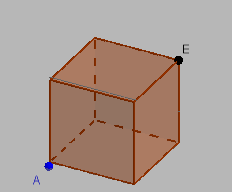
\includegraphics[width=0.5\textwidth]{01}
\vvs
\ep

\end{document}